% Stage 2 report: design approach, tools, the reference setup, steady-state calibration and the
% steady-state predictor. Compile from this folder: pdflatex stage2.tex (twice).
\documentclass[11pt,a4paper]{article}
\usepackage[margin=2.2cm]{geometry}
\usepackage[T1]{fontenc}
\usepackage{lmodern}
\usepackage{amsmath}
\usepackage{graphicx}
\usepackage[export]{adjustbox}
\usepackage{booktabs}
\usepackage{array}
\usepackage{enumitem}
\usepackage{xcolor}
\usepackage{caption}
\usepackage{float}
\usepackage{tikz}
\usetikzlibrary{positioning,arrows.meta,fit}
\usepackage[section]{placeins}
\usepackage[hidelinks]{hyperref}
\graphicspath{{../experiments/}{../data/sample_dataset/2D_floorplans/}}
\setlist{itemsep=1pt,topsep=3pt}
\setlength{\parindent}{0pt}
\setlength{\parskip}{5pt}
\captionsetup{font=small,labelfont=bf}
\newcommand{\us}{\,$\mu$s}
\newcommand{\degC}{\,\textdegree C}
\setcounter{tocdepth}{1}

\begin{document}

\begin{center}
{\LARGE\bfseries Lightweight Temperature Predictor:}\\[4pt]
{\Large\bfseries TapaSense}\\[8pt]
{\large Stage 2 Report: Design, Tools and the Steady-State Predictor}\\[6pt]
Ethan Bobby Kurien \quad Kaivalya Mase
\end{center}

\tableofcontents

%=====================================================================
\section{Introduction}\label{sec:intro}
A modern chip has several cores. When they work hard they heat up, and if they get too hot they
slow down, wear out faster or fail. The chip's dynamic thermal management (DTM) keeps them under a
limit by lowering frequency and voltage \cite{skadron03}. To decide well it needs to know how hot
each core is, and ideally how hot it will be a few milliseconds from now
\cite{coskun09}.

HotSpot \cite{hotspot,hotspot6}, a widely used research simulator, computes chip temperatures
accurately, but far too slowly for this. One steady-state answer takes about a quarter of a
second, while DTM needs an answer every millisecond.

\textbf{The assignment.} \emph{Develop a lightweight temperature predictor in two stages.
Calibration (one-time per floorplan): tune the predictor's coefficients for the given floorplan
with heterogeneous cores. Prediction: predict the temperature (steady state or transient) for a
given power input.}

This report covers the design of the whole system, the tools we used, the HotSpot reference
setup, and steady-state prediction: calibration, the predictor, and its evaluation against
HotSpot.

%=====================================================================
\section{Design approach}

\subsection{Steady-state and transient prediction}
The assignment asks for two kinds of prediction, and we plan one predictor for each.
\begin{itemize}
  \item \textbf{Steady state.} The power is held constant until the temperatures stop changing,
        which takes seconds. The answer depends only on the present power, so the predictor is
        a fixed formula from power to temperature (Equation~\eqref{eq:s1} below). It answers
        ``how hot will this power setting eventually get'', for example when choosing a safe
        operating point or deciding which core gets a task.
  \item \textbf{Transient.} The temperature over time as the power changes from one millisecond
        to the next. The die and package store heat (thermal capacitance), so the temperature
        lags behind the power and depends on its history. A transient predictor therefore needs
        a state (the current temperatures) and the chip's time constants, not just a fixed
        formula. It is what DTM uses to forecast a few milliseconds ahead.
\end{itemize}
Both use the same idea of a one-time calibration on planned HotSpot runs, and both rely on HotSpot
being linear. The steady-state prediction is also the value a transient prediction settles to
when the power stops changing. \textbf{So far we have built and evaluated the steady-state
predictor}; the transient predictor is the next stage.

\subsection{Two stages}
The predictor is split into a calibration stage that runs once per floorplan and a prediction
stage that runs many times (Figure~\ref{fig:pipeline}).

\begin{figure}[H]
\centering
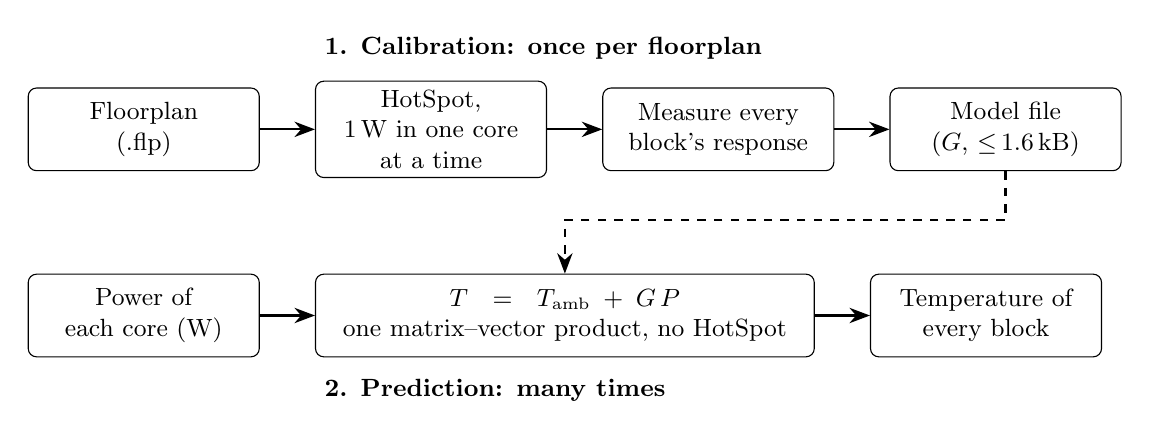
\begin{tikzpicture}[
  box/.style={draw, rounded corners=3pt, align=center, minimum height=1.05cm, font=\small,
              text width=2.7cm, fill=white},
  arr/.style={-{Stealth[length=2.6mm]}, thick},
  lab/.style={font=\small\bfseries}]
  \node[box] (flp) {Floorplan\\(.flp)};
  \node[box, right=0.7cm of flp] (hs) {HotSpot,\\1\,W in one core\\at a time};
  \node[box, right=0.7cm of hs] (g) {Measure every\\block's response};
  \node[box, right=0.7cm of g] (npz) {Model file\\($G$, $\le$\,1.6\,kB)};
  \node[box, below=1.3cm of flp] (p) {Power of\\each core (W)};
  \node[box, right=0.7cm of p, text width=6.1cm] (pred) {$T = T_\text{amb} + G\,P$\\ one matrix--vector product, no HotSpot};
  \node[box, right=0.7cm of pred] (t) {Temperature of\\every block};
  \draw[arr] (flp) -- (hs); \draw[arr] (hs) -- (g); \draw[arr] (g) -- (npz);
  \draw[arr] (p) -- (pred); \draw[arr] (pred) -- (t);
  \draw[arr, dashed] (npz.south) -- ++(0,-0.62) -| (pred.north);
  \node[lab, above=0.15cm of hs.north west, anchor=south west] {1. Calibration: once per floorplan};
  \node[lab, below=0.15cm of pred.south west, anchor=north west] {2. Prediction: many times};
\end{tikzpicture}
\caption{The two stages. Calibration runs HotSpot a few times with planned inputs and stores the
coefficients; prediction uses only the coefficients.}
\label{fig:pipeline}
\end{figure}

\subsection{Why a linear model can be exact}\label{sec:linear}
HotSpot models the die and its package (silicon, thermal paste, heat spreader, heat sink) as a
large network of thermal resistances and capacitances \cite{skadron03,hotspot}. Without
temperature-dependent leakage this network is \emph{linear}: if the power doubles, every
temperature rise doubles, and the rises caused by different cores add up. It follows that the
steady temperature is
\begin{equation}
  T_i = T_\text{amb} + \sum_{j=1}^{N} G_{ij}\,P_j
  \qquad\text{or}\qquad T = T_\text{amb} + G\,P ,
  \label{eq:s1}
\end{equation}
where $P_j$ is the power of core $j$, $T_\text{amb}$ the ambient temperature, and $G_{ij}$ the
rise of block $i$ per watt in core $j$ (in K/W). $G_{ii}$ is self-heating; $G_{ij}$ with
$i\neq j$ is coupling. Putting 1\,W into core $j$ and nothing elsewhere gives
$T - T_\text{amb} = G\,e_j$, which is exactly column $j$ of $G$.

\textbf{Worked example.} Two cores: a little core (1) and a big core (2). With values in the range
we measured, the little core self-heats 1.5\,K/W, the big core 0.6\,K/W, and each warms the other
by 0.3\,K/W:
\[
G = \begin{pmatrix} 1.5 & 0.3 \\ 0.3 & 0.6 \end{pmatrix}\text{K/W},\quad
P = \begin{pmatrix} 8 \\ 20 \end{pmatrix}\text{W}
\;\Rightarrow\;
G\,P = \begin{pmatrix} 1.5\cdot 8 + 0.3\cdot 20 \\ 0.3\cdot 8 + 0.6\cdot 20 \end{pmatrix}
     = \begin{pmatrix} 18.0 \\ 14.4 \end{pmatrix}\text{K}.
\]
With $T_\text{amb} = 45$\degC, the little core reaches 63.0\degC\ and the big core 59.4\degC. The
little core ends up hotter on less than half the power, because it packs more watts into each
square millimetre. This is the heterogeneity effect we see on every floorplan.

\subsection{Steady-state models}\label{sec:models}
Both models below predict with Equation~\eqref{eq:s1}. They differ only in where $G$ comes from.

\textbf{S0, power blurring (no calibration) \cite{blurring}.} Idea: heat from a small source
spreads out the same way on every chip, so one measured spreading pattern can be reused.
\begin{enumerate}
  \item \emph{Once, for all floorplans:} one HotSpot run with a tiny 1\,W source in the middle of
        a large 28\,mm die. The temperature rise against distance from the source is a generic
        kernel $K(r)$ (Figure~\ref{fig:kernel}).
  \item \emph{For a new floorplan:} to get column $j$, spread 1\,W evenly over the grid cells of
        core $j$. Every heated cell $s$ warms every cell $q$ by its power times $K(|q-s|)$, and
        the contributions add up. Averaging the result over the cells of block $i$ gives
        $G_0[i,j]$.
\end{enumerate}
S0 never runs HotSpot on the target floorplan, so comparing it with S1 shows what calibration
adds. Its weakness is that one kernel ignores the die edges and the die size.

\textbf{S1, influence matrix (calibrated).} $G$ is measured on the floorplan itself.
\begin{itemize}
  \item \emph{Calibration.} For each core $j = 1,\dots,N$, run HotSpot to steady state with 1\,W
        in core $j$ and 0\,W everywhere else, and record the temperature of every block. Then
        \[ G[:,j] = T_\text{HotSpot}(\text{1\,W in core } j) - T_\text{amb}. \]
        That is $N$ steady runs and no fitting: each column is copied straight from one run.
  \item \emph{Why it is exact.} Any power vector is a sum of unit vectors,
        $P = \sum_j P_j\, e_j$. Because HotSpot is linear (verified in
        Section~\ref{sec:linearity}), its response is the same sum of the unit responses,
        $\sum_j P_j\, G e_j = G P$. No approximation is involved.
  \item \emph{Which temperatures are predicted.} S1 predicts the temperature of every block of
        the floorplan. So $G$ has one row per block ($n$ rows, the number of blocks) and one
        column per core ($N$ columns, the number of power inputs). On the given floorplans
        $N = 8$, and $n$ ranges from 9 to 25 depending on the layout.
\end{itemize}
S1 predicts each block's \emph{average} temperature. Section~\ref{sec:hotspot} extends it to the
hottest point inside each core, using the same calibration runs.

\subsection{Evaluation methodology}\label{sec:eval}
\begin{itemize}
  \item \textbf{Reference:} HotSpot 6.0 \cite{hotspot6} grid model with $64\times64$ cells, the
        given layer stack (silicon 150\,$\mu$m, thermal paste 20\,$\mu$m), HotSpot's standard
        package (30\,mm spreader, 60\,mm heat sink, 0.1\,K/W convection), ambient 45\degC.
  \item \textbf{Test data is never used for calibration.} Calibration uses only unit-power runs.
        Tests use the given nominal and maximum power and 300 random power vectors per floorplan
        (big cores 10--20\,W, little cores 5--10\,W, uniform).
  \item \textbf{Accuracy:} with $e_i = T_{\text{model},i} - T_{\text{HotSpot},i}$ over the cores:
        mean $|e_i|$, worst $|e_i|$, the error in the chip's peak temperature, and the share of
        cases where the model picks HotSpot's hottest core.
  \item \textbf{Model size:} stored coefficients $\times$ 8 bytes (64-bit numbers) unless stated.
\end{itemize}

\textbf{Targets} were set before any experiment: mean error $\le 0.1$\,K, peak error
$\le 0.2$\,K, hottest core right $\ge 99$\,\%, $\le 20$\us\ per prediction and model $\le 5$\,kB.
For accuracy, learned surrogates trained on HotSpot data reach 0.44--0.93\,K RMSE when the
layout, materials or boundary conditions change \cite{thermbench}. Since our predictor is
calibrated on the floorplan it predicts, we aimed an order of magnitude tighter. For time and
size, a run-time predictor has to run at every DTM interval (milliseconds) without adding
noticeable overhead \cite{coskun09,zhang18}, so we aimed for microseconds and a few kilobytes.

%=====================================================================
\section{Tools and frameworks}\label{sec:tools}
HotSpot 6.0 \cite{hotspot6} (grid model, SuperLU solver) is the reference simulator, run under
Ubuntu on WSL. The predictor, the calibration and all experiments are written in Python 3 with
NumPy and SciPy, and the figures are made with Matplotlib.

\subsection{A precision patch for HotSpot}
HotSpot prints temperatures rounded to 0.01\,K. Our predictor's errors are far smaller than that,
so the stock output cannot measure them: every error below 0.005\,K would look like zero or like
rounding noise. We patched a copy of HotSpot's output code to print 6 decimals (1\,$\mu$K). The
computation itself is unchanged, and the original HotSpot stays untouched.

%=====================================================================
\section{Data}

\begin{figure}[H]
  \centering
  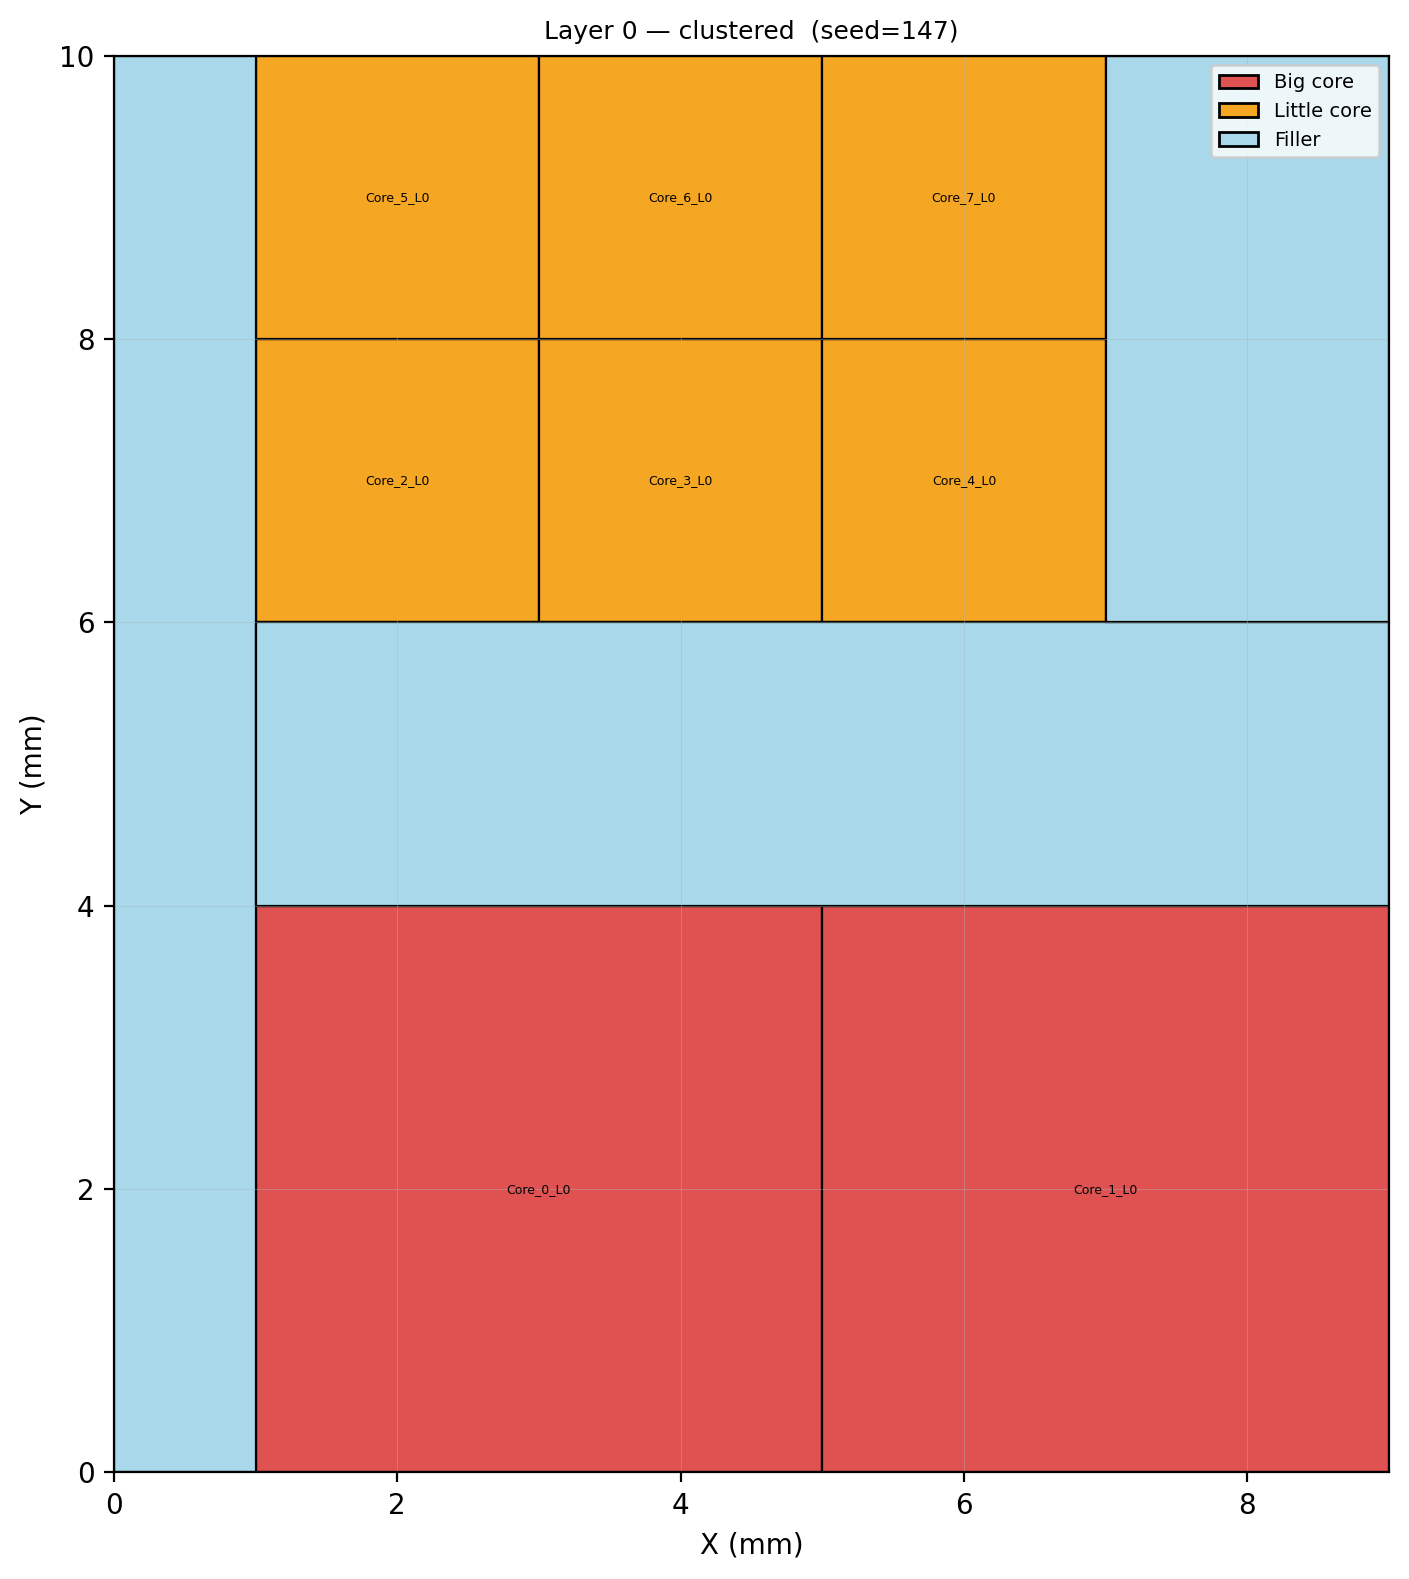
\includegraphics[height=3.6cm]{Style_1/fp_001/fp_001_layer_0.png}\hfill
  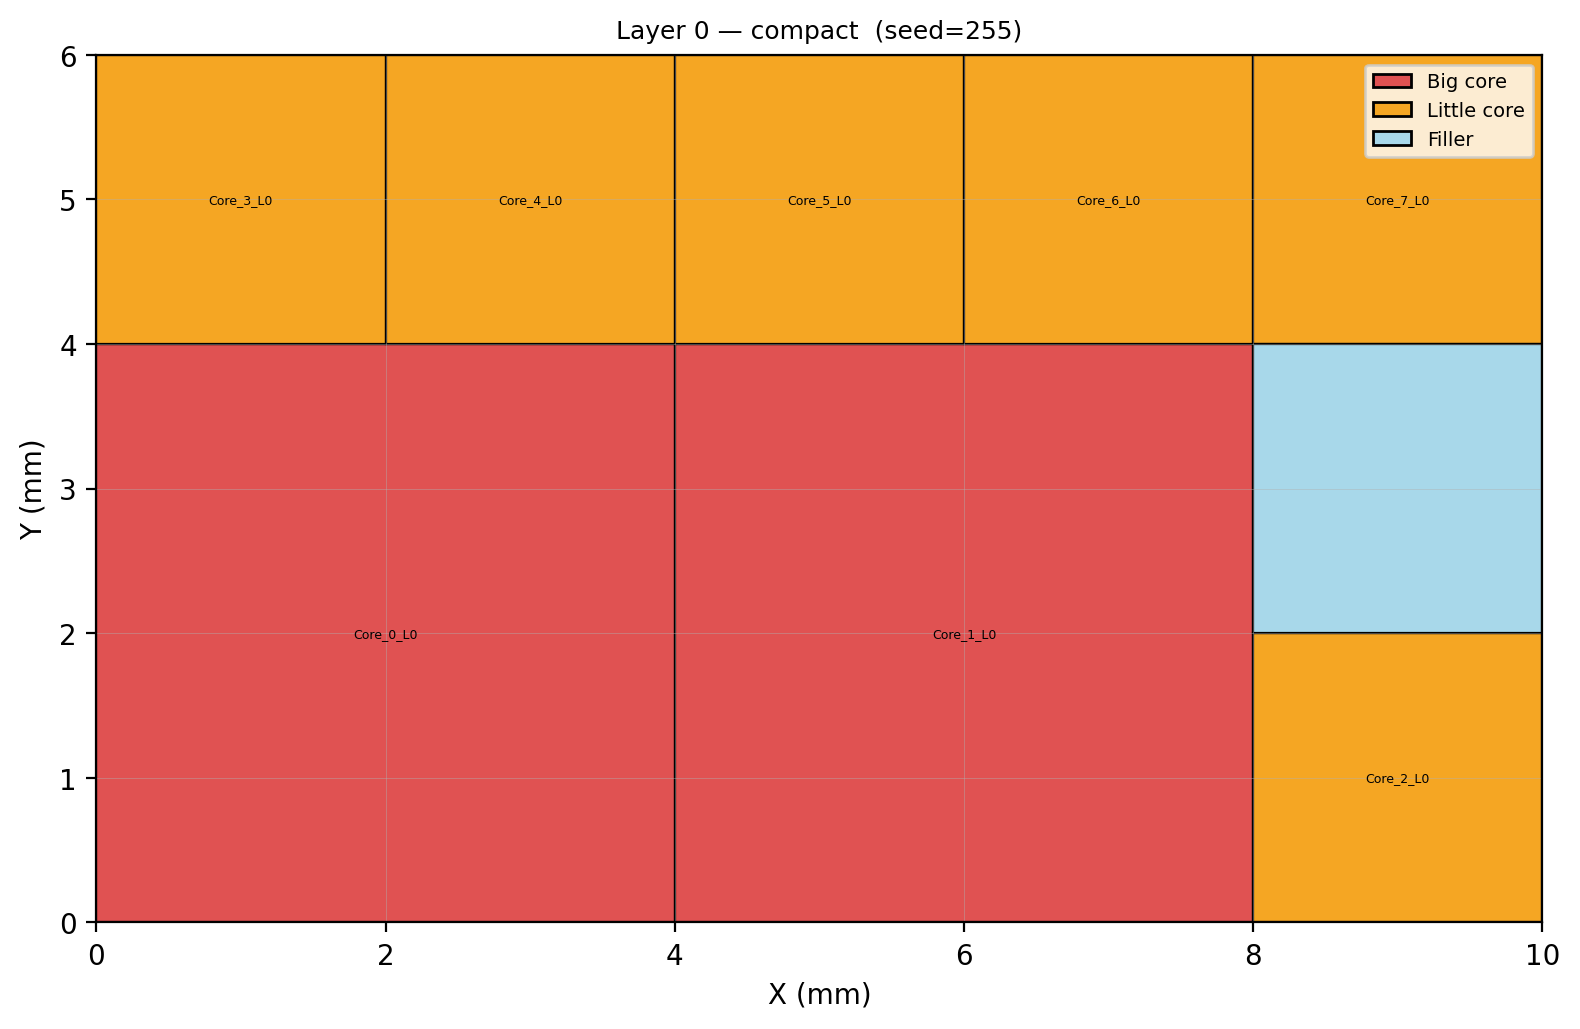
\includegraphics[height=3.6cm]{Style_2/fp_004/fp_004_layer_0.png}\hfill
  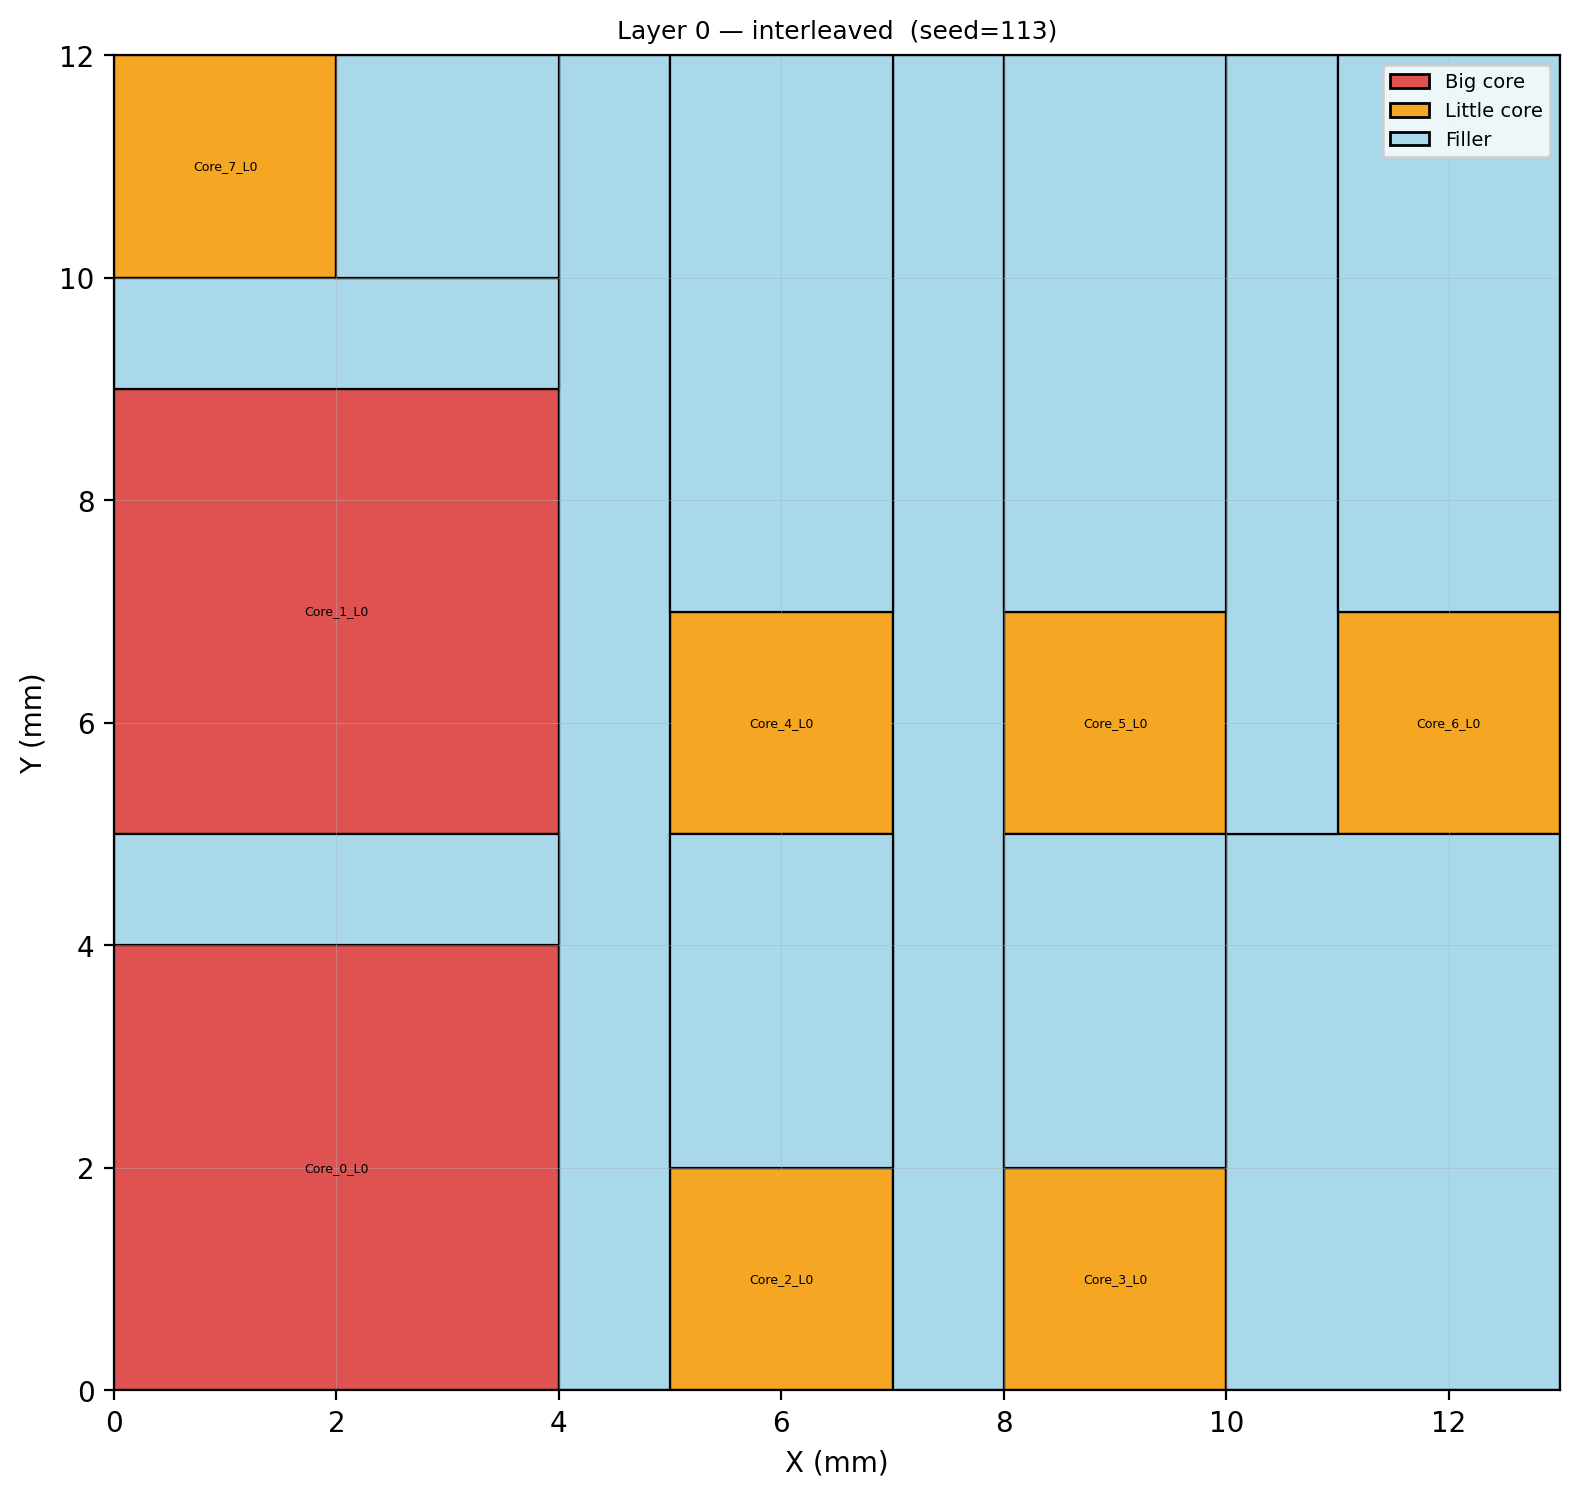
\includegraphics[height=3.6cm]{Style_3/fp_002/fp_002_layer_0.png}\hfill
  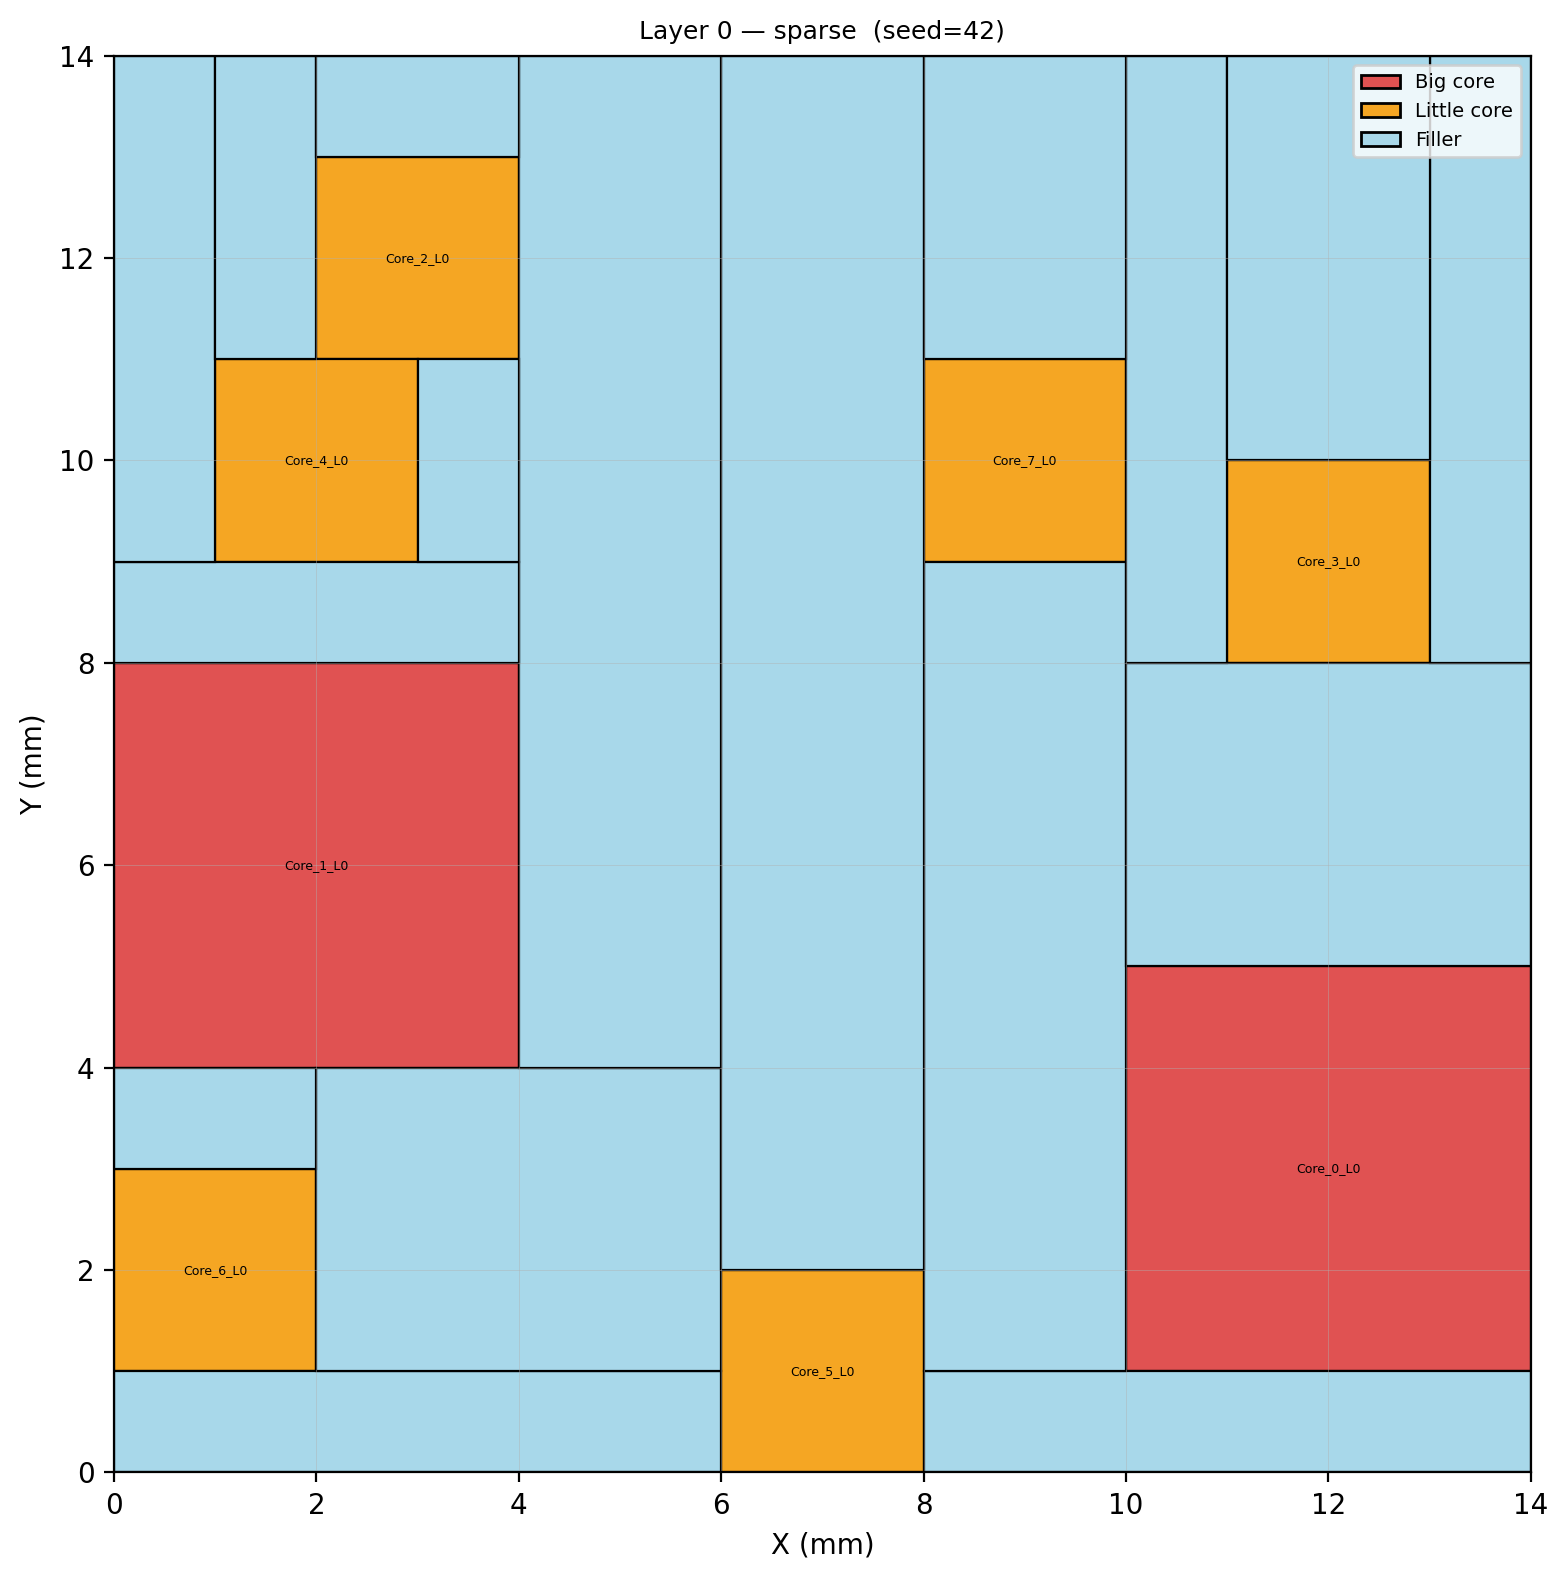
\includegraphics[height=3.6cm]{Style_4/fp_001/fp_001_layer_0.png}
  \caption{One floorplan per style, from left to right Style 1 to Style 4 (red = big core,
  orange = little core, blue = FILL). Every floorplan has 2 big cores (4$\times$4\,mm) and 6
  little cores (2$\times$2\,mm); the rest of the die is white space with no power.}
  \label{fig:ta}
\end{figure}

\begin{center}
\small
\begin{tabular}{@{}l p{9.6cm} c@{}}
\toprule
Set & Description & Floorplans \\
\midrule
Style 1 & Big cores together, little cores in a cluster; dies 9$\times$10 to 16$\times$8\,mm & 3 \\
Style 2 & Tightly packed, small dies (62--93\,\% covered by cores) & 5 \\
Style 3 & At least 1\,mm between cores, long or larger dies & 5 \\
Style 4 & Same 14$\times$14\,mm die, cores scattered (29\,\% covered) & 10 \\
HET-A & Our own heterogeneous layout with L2 and network-on-chip blocks & 1 \\
HOM-16, HOM-64 & Synthetic grids of 16 and 64 identical 2$\times$2\,mm cores, for compression tests & 2 \\
Generated & 13 per style, same cores and file format & 52 \\
\bottomrule
\end{tabular}
\end{center}

\textbf{Power.} Nominal (the given values): big 20\,W, little 8\,W, 88\,W per chip. Maximum: big
20\,W, little 10\,W. Random test vectors: big 10--20\,W, little 5--10\,W.

\begin{figure}[H]
  \centering
  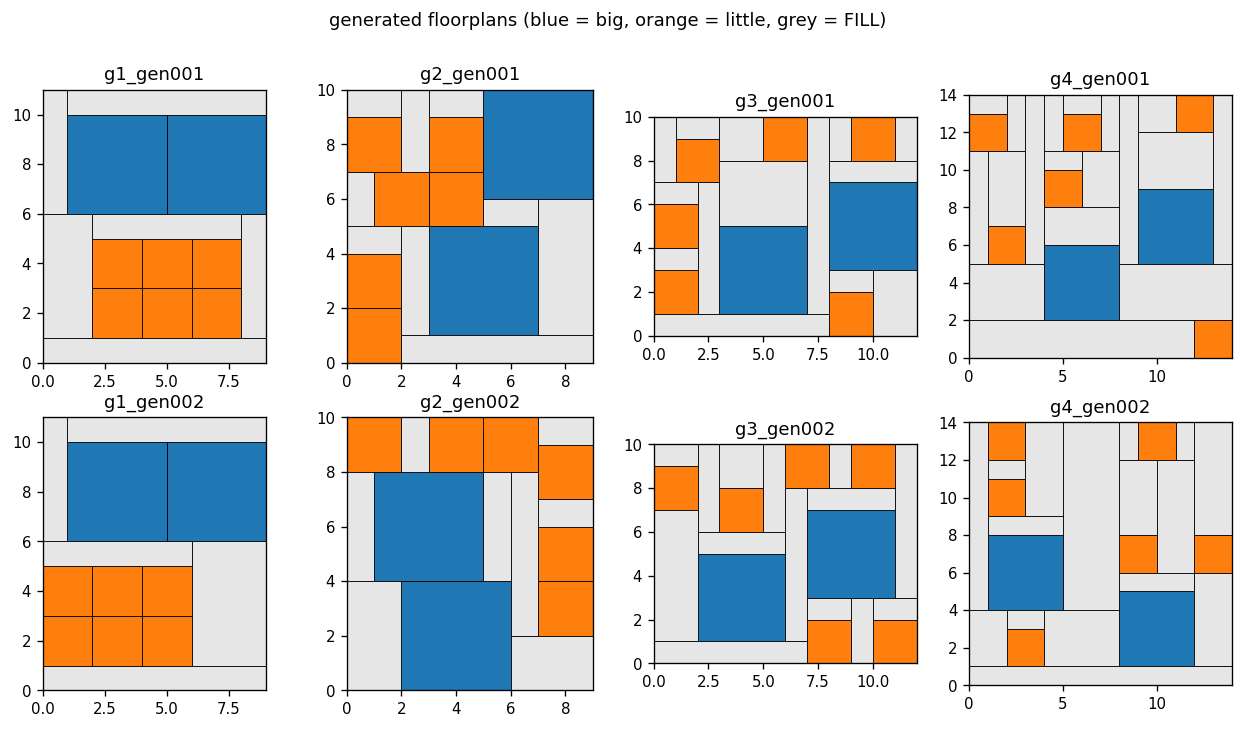
\includegraphics[width=0.8\linewidth]{P0-5d_generated_floorplans/results/examples.png}
  \caption{Generated floorplans, two per style (blue = big, orange = little, grey = FILL). They
  behave like the given floorplans of the same style, and we use them to check the predictor on
  floorplans it was not developed on (Figure~\ref{fig:s1maps}).}
\end{figure}

%=====================================================================
\section{Establishing the reference}
Before building a predictor we checked that the reference behaves as the theory says and chose its
settings.

\subsection{Is HotSpot linear?}\label{sec:linearity}
On one floorplan per style (Figure~\ref{fig:ta}) we scaled the power by 0.5, 2 and 3, ran zero power, and ran the big
and little cores separately and added the results; we repeated the checks on a 0.5\,s transient
trace.

\begin{center}
\small
\begin{tabular}{@{}l c@{}}
\toprule
Check & Largest deviation \\
\midrule
Scaling ($\times 0.5$, $\times 2$, $\times 3$) & $\le 3\times10^{-6}$\,K \\
Superposition (big + little run separately) & $\le 1\times10^{-6}$\,K \\
Zero power & exactly 45\degC \\
1\,W vs 10\,W calibration step & identical after scaling \\
\bottomrule
\end{tabular}
\end{center}

\begin{figure}[H]
  \centering
  \adjincludegraphics[trim={0 0 {.5\width} 0}, clip, width=0.5\linewidth]{P0-2_linearity/results/transient_linearity.png}
  \caption{One core's temperature rise on a transient trace for power $P$, for $P_A + P_B$ run
  separately and added, and for $2P$ halved. The three curves coincide.}
\end{figure}

HotSpot is linear and additive, and zero power gives exactly the ambient temperature, so Equation~\eqref{eq:s1} needs no offset term.

\subsection{Block model or grid model?}\label{sec:blockgrid}
HotSpot can treat each block as one node (block model) or divide the die into a grid of cells.
The block model is known to lose accuracy on large or elongated blocks \cite{huang07}.

\begin{center}
\small
\begin{tabular}{@{}l c c c@{}}
\toprule
Floorplan & Block vs grid & Grid $64^2$ vs $128^2$ & Hottest cell $-$ core average \\
\midrule
s1\_fp001 & 1.89\,K & 0.03\,K & 3.33\,K \\
s2\_fp004 & 1.14\,K & 0.01\,K & 3.99\,K \\
s3\_fp002 & 3.72\,K & 0.13\,K & 3.95\,K \\
s4\_fp001 & 5.36\,K & 0.15\,K & 3.79\,K \\
\bottomrule
\end{tabular}
\end{center}

\begin{figure}[H]
  \centering
  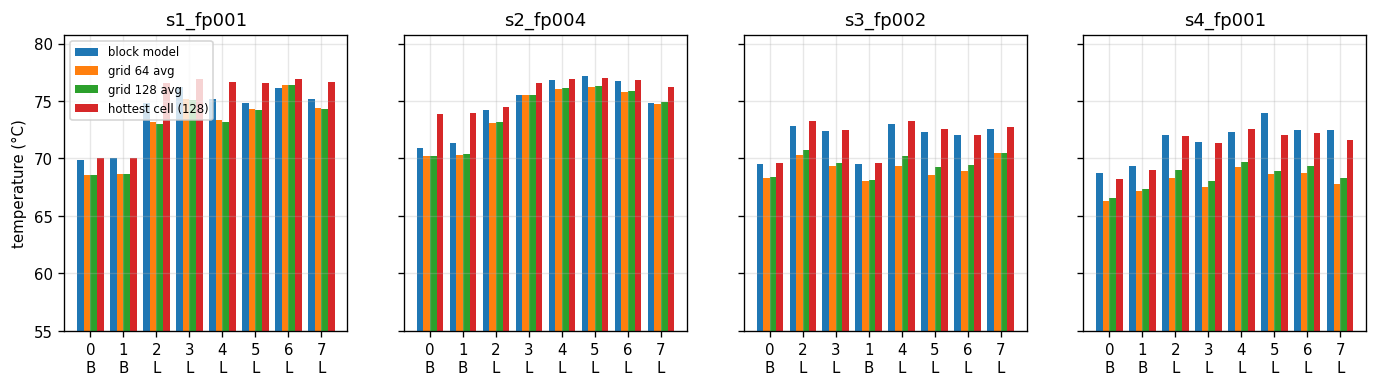
\includegraphics[width=\linewidth]{P0-3_block_vs_grid/results/per_core.png}
  \caption{Per-core temperature at nominal power on one floorplan per style: block model, grid
  $64\times64$ average, grid $128\times128$ average, and the hottest $128\times128$ cell
  (B = big, L = little core).}
\end{figure}

\begin{itemize}
  \item The block model is 1--5\,K off the grid model, worst on large sparse dies. We use the grid
        model, as the given setup does.
  \item $64\times64$ is fine enough: going to $128\times128$ changes core averages by at most
        0.15\,K.
  \item The hottest cell is 3.3--4\,K above its core's average, so a limit on core averages lets
        the real peak run about 4\,K hotter (addressed in Section~\ref{sec:hotspot}).
\end{itemize}

\begin{figure}[H]
  \centering
  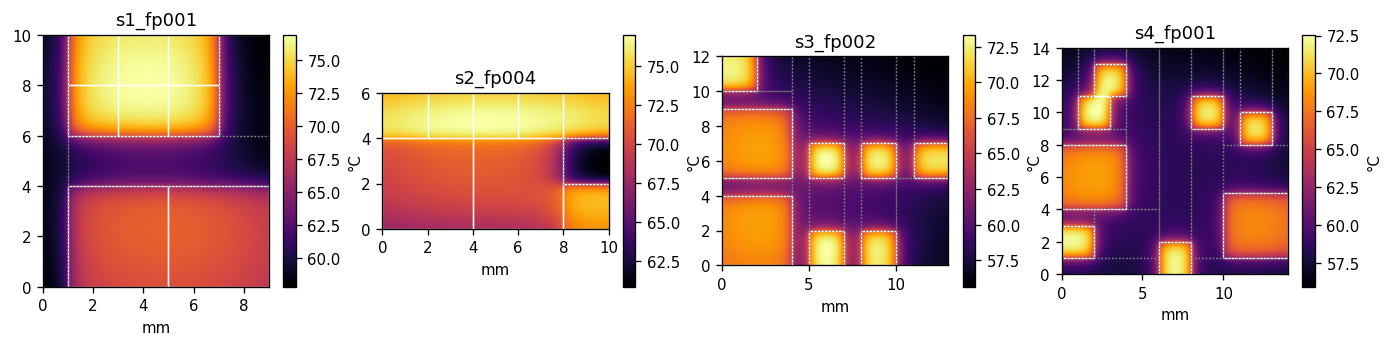
\includegraphics[width=0.9\linewidth]{P0-3_block_vs_grid/results/maps_128.png}
  \caption{$128\times128$ temperature maps at nominal power. Heat concentrates in the middle of
  each core, and small little cores form the sharpest peaks.}
\end{figure}

\subsection{How hot do the given floorplans run?}
All 23 floorplans run unchanged. The hottest core reaches 69--77\degC\ at nominal power and
73--83\degC\ at maximum power. \textbf{A little core is the hottest core on every floorplan}: it has
1.6$\times$ the power density of a big core. Packing matters more than die size alone.

\begin{figure}[H]
  \centering
  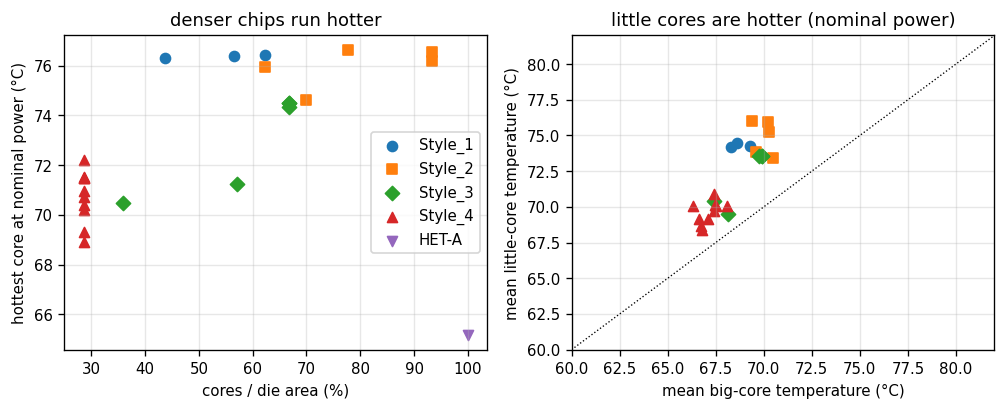
\includegraphics[width=0.75\linewidth]{P0-5_ta_floorplans/results/peak_vs_density.png}
  \caption{Peak temperature against how densely the die is covered by cores. Denser floorplans run
  hotter; little cores run hotter than big cores.}
\end{figure}

%=====================================================================
\section{Steady-state calibration}

\subsection{Procedure and cost}
For each of the 24 floorplans (23 given plus HET-A), with $N = 8$ cores: 8 steady HotSpot runs, each
with 1\,W in one core and 0\,W elsewhere. Run $j$ gives column $j$ of $G$; the full $64\times64$
map of the same runs gives the cell coefficients used for hot spots (Section~\ref{sec:hotspot}).

\begin{center}
\small
\begin{tabular}{@{}l c c@{}}
\toprule
Style & Floorplans & Calibration time (8 steady runs), mean \\
\midrule
Style 1 & 3 & 4.6\,s \\
Style 2 & 5 & 4.4\,s \\
Style 3 & 5 & 4.2\,s \\
Style 4 & 10 & 4.2\,s \\
\bottomrule
\end{tabular}
\end{center}
Calibration costs about 4.3\,s of HotSpot time per floorplan; turning the runs into $G$ is a copy
of the results. The cost does not depend on the layout, because the grid is always $64\times64$
and every floorplan has 8 cores.

\subsection{What $G$ looks like}
\begin{figure}[H]
  \centering
  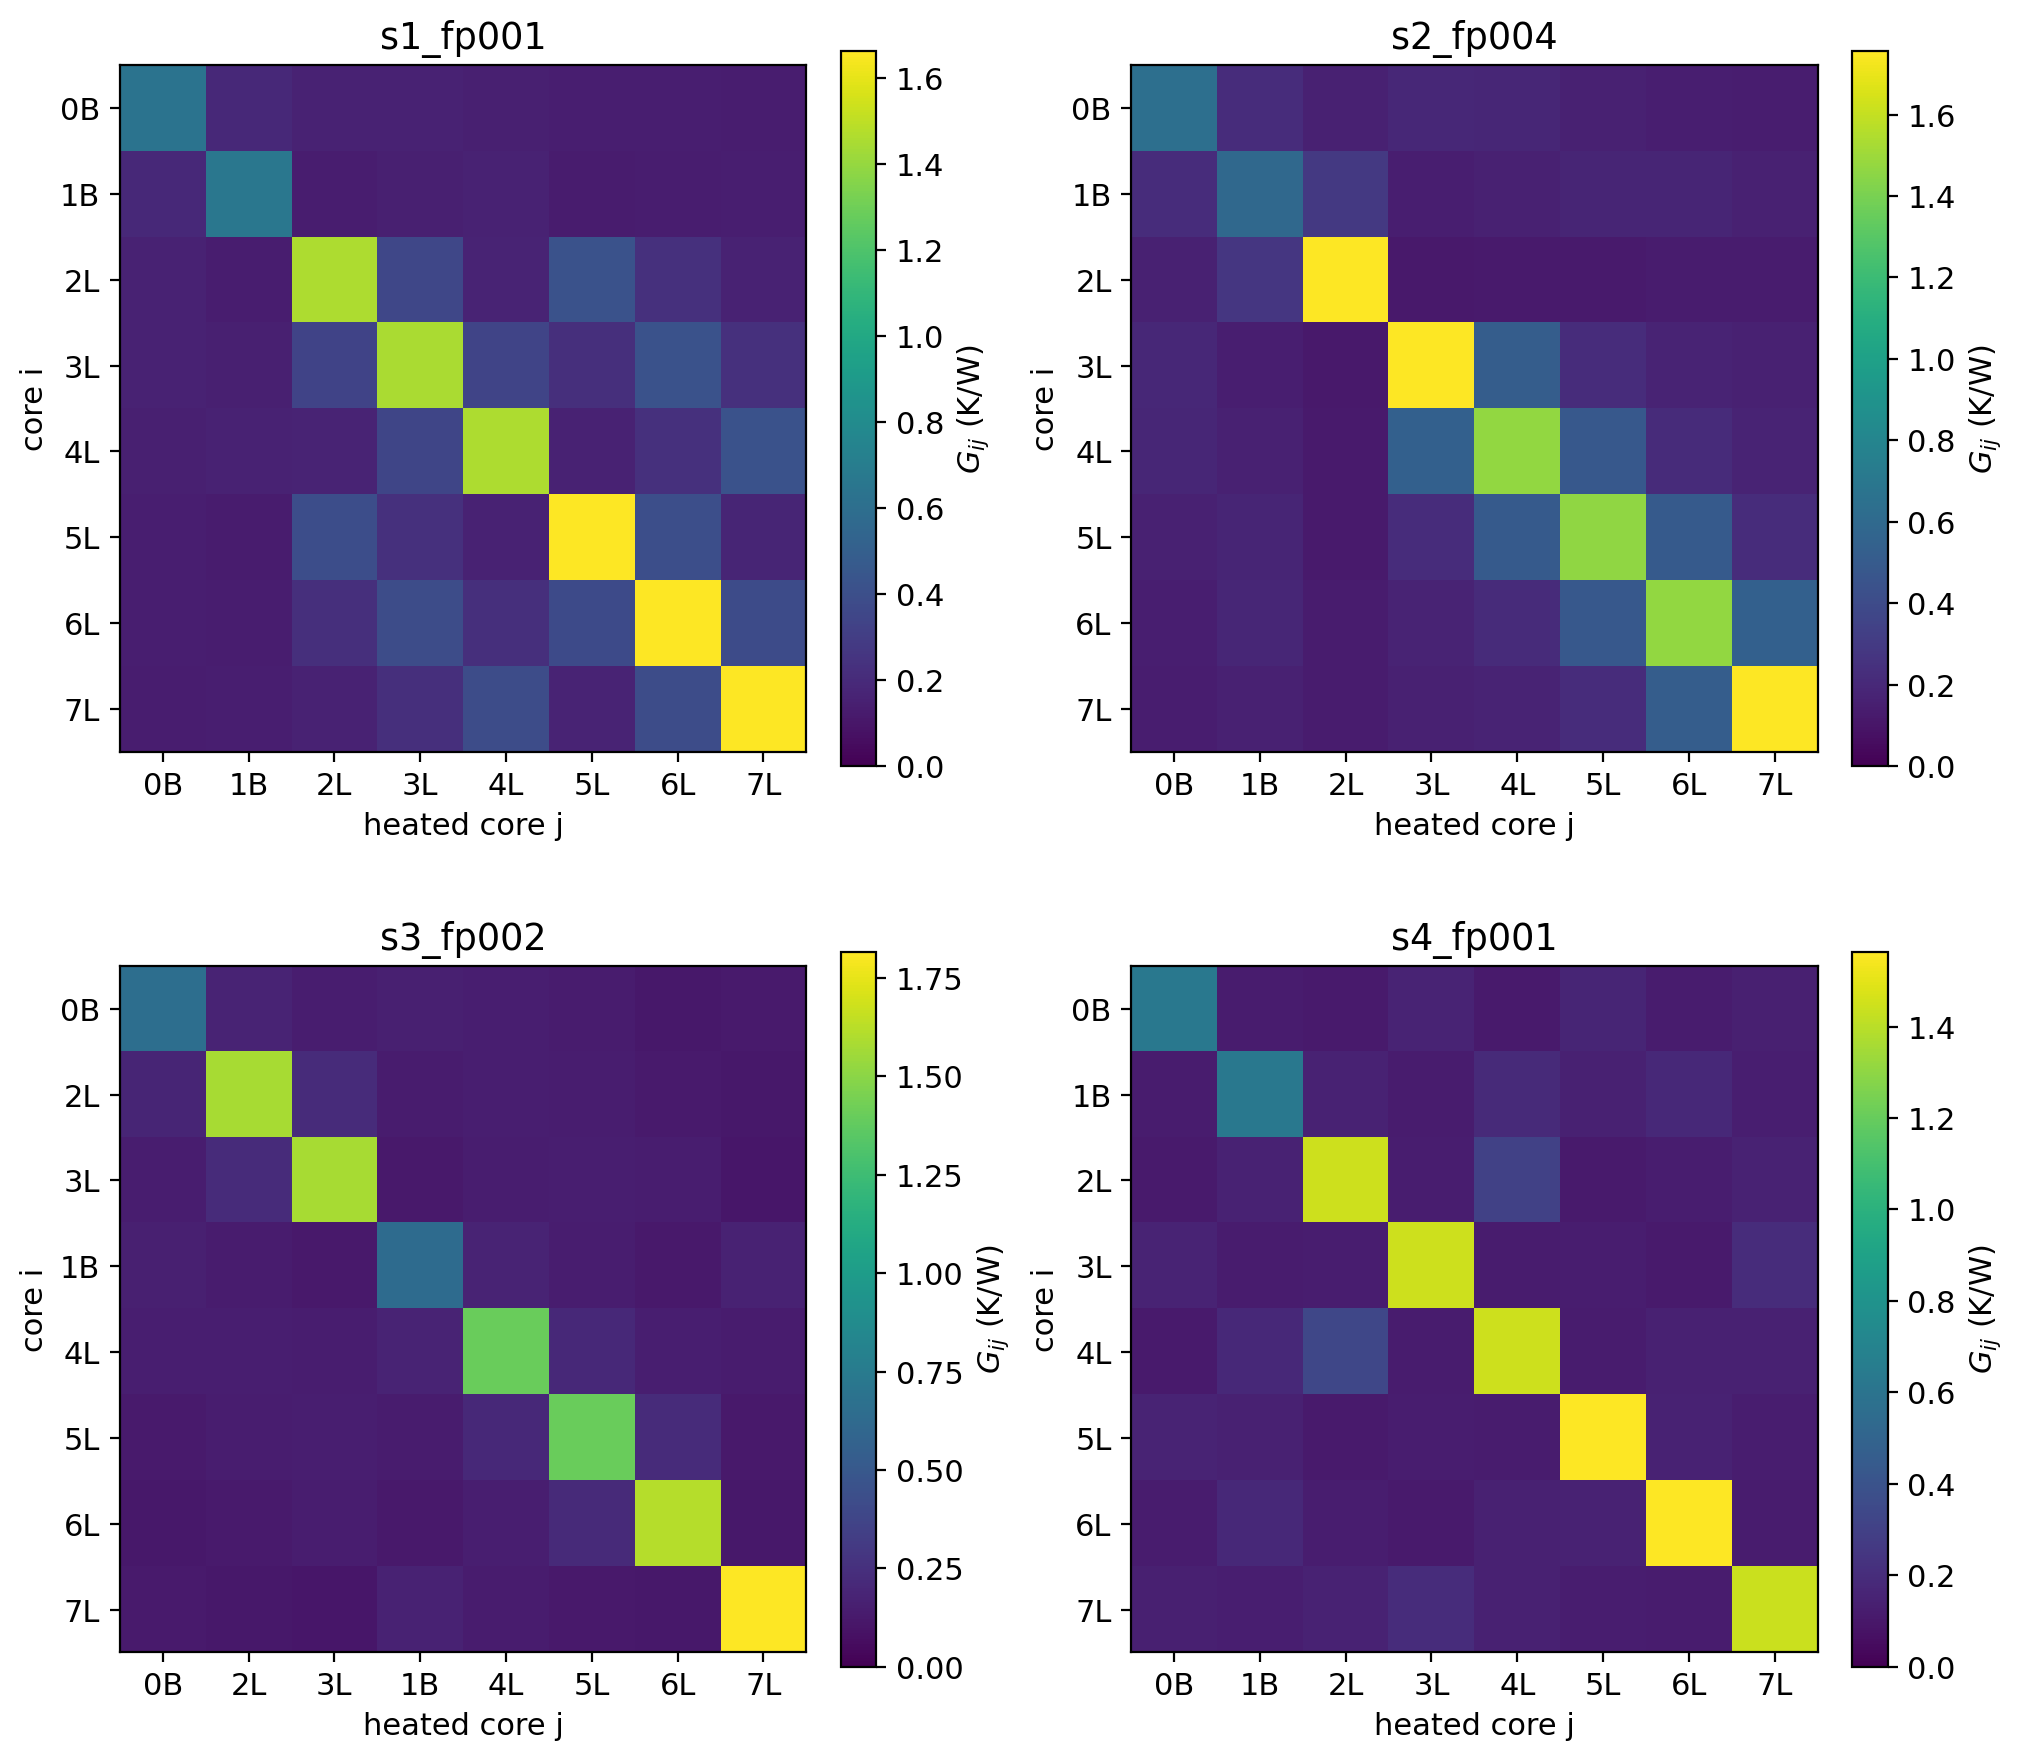
\includegraphics[width=0.85\linewidth]{P1-1_step_calibration/results/G_heatmaps_stage2.png}
  \caption{Calibrated $G$ (K/W) for one floorplan per style (B = big, L = little core). The bright
  diagonal entries are the self-heating of the little cores; off-diagonal entries are coupling
  between cores.}
\end{figure}

\begin{itemize}
  \item A little core heats itself 2.4$\times$ as much per watt as a big core (about 1.5 vs
        0.62\,K/W).
  \item Cores on a die edge heat themselves more (up to 1.85\,K/W), because heat cannot spread
        outwards.
  \item \textbf{Every core warms every other core, even distant ones.} The smallest off-diagonal
        entry of $G$ is 0.10--0.14\,K/W, depending on the floorplan: 1\,W in any core raises
        every other core by at least that much. This floor comes from the package. All the heat
        leaves through the same heat spreader and heat sink, which warm up as a whole and lift
        the temperature of the entire die. Nearby cores add local coupling on top of this floor
        (up to 0.63\,K/W for cores 2\,mm apart, Section~\ref{sec:layout}).
\end{itemize}

%=====================================================================
\section{Is per-floorplan calibration needed?}\label{sec:calneeded}
Calibration costs HotSpot runs on every new floorplan. Could a predictor that never runs HotSpot on
the target do as well? The given dataset is well suited to this question: the cores and power are the
same on every floorplan, and only the layout differs.

We tested calibration-free methods on 6{,}946 unseen HotSpot runs (the nominal and maximum power
and 300 random vectors on each of the 23 given floorplans).
\begin{itemize}
  \item \textbf{Borrow $G$ from another floorplan of the same style:} on Style~4 the die, cores
        and power are identical and only the core positions differ, so this is the most
        favourable case for reuse. We use every other Style~4 floorplan's $G$ (all 90 pairs),
        cores matched by type.
  \item \textbf{Borrow $G$ from another style:} the $G$ of s1\_fp001 (Style~1) applied to each of
        the 20 floorplans of Styles 2--4, cores matched by type.
  \item \textbf{S0 power blurring:} the generic heat-spread kernel of Section~\ref{sec:models}
        (Figure~\ref{fig:kernel}). It gets the overall shape of $G$ right but ignores die edges
        and die size.
\end{itemize}

\begin{figure}[H]
  \centering
  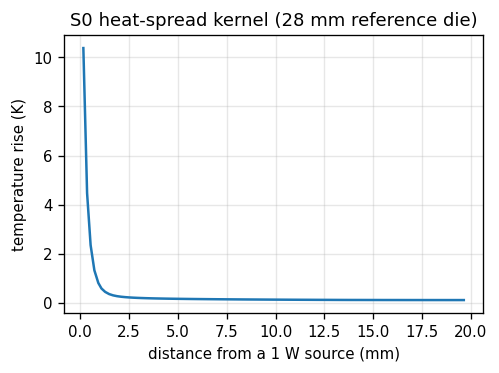
\includegraphics[width=0.5\linewidth]{P1-3_is_calibration_needed/results/s0_kernel.png}
  \caption{The generic heat-spread kernel used by S0: rise against distance from a 1\,W source on
  a 28\,mm reference die. It falls steeply within 2\,mm and then levels off at the package term.}
  \label{fig:kernel}
\end{figure}

\begin{center}
\small
\begin{tabular}{@{}l c c c c@{}}
\toprule
Method & Runs on target & Mean error & Worst error & Hottest core right \\
\midrule
\textbf{S1, calibrated} & \textbf{8} & \textbf{0.000007\,K} & \textbf{0.00003\,K} & \textbf{100\,\%} \\
S0 power blurring & 0 & 0.76\,K & 5.2\,K & 71\,\% \\
Borrow $G$, same style (Style 4) & 0 & 1.11\,K & 5.2\,K & 60\,\% \\
Borrow $G$, another style (s1\_fp001's) & 0 & 2.79\,K & 12.1\,K & 46\,\% \\
\bottomrule
\end{tabular}
\end{center}

\begin{figure}[H]
  \centering
  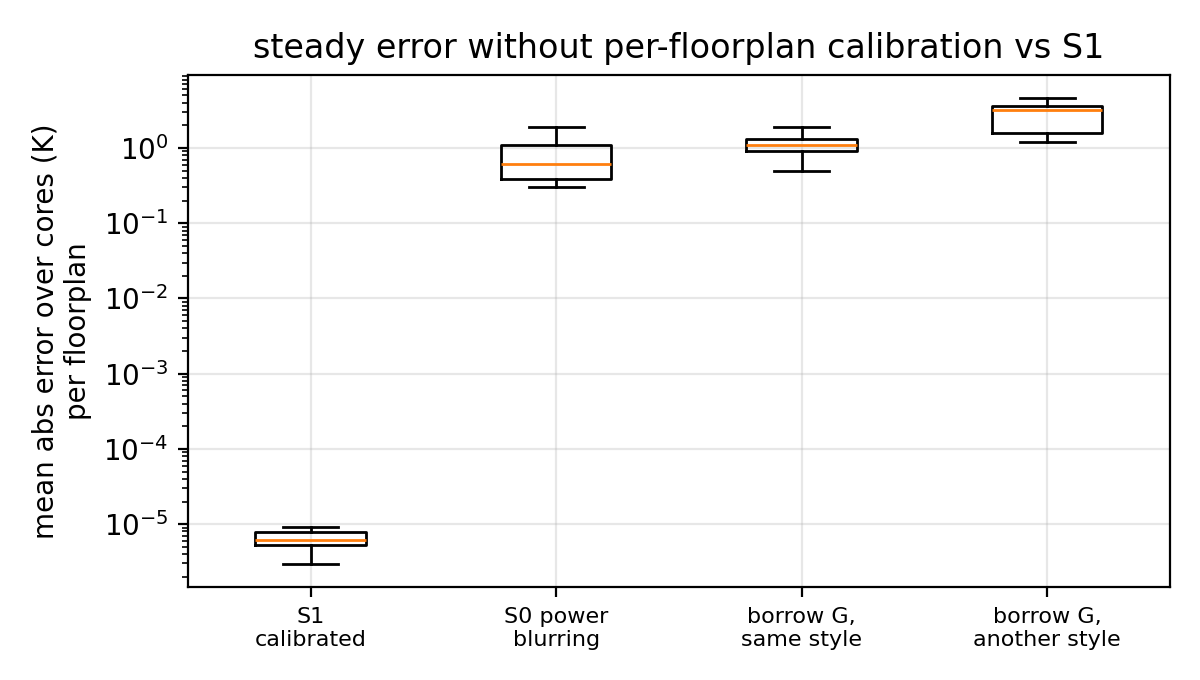
\includegraphics[width=0.6\linewidth]{P1-3_is_calibration_needed/results/error_by_method_stage2.png}
  \caption{Comparing borrowed strategies against calibration.}
\end{figure}

\textbf{Calibration is needed.} Without it, errors are 0.8--2.8\,K on average and 5--12\,K in the
worst case, and the wrong core is named hottest in 29--54\,\% of cases. Even within one style, on
Style~4 where only the core positions differ, borrowing another floorplan's $G$ is 1.1\,K off on
average; borrowing across styles is 2.8\,K off. Four seconds of calibration beat every shortcut by
a factor of more than 10{,}000.

%=====================================================================
\section{The steady-state predictor}\label{sec:predictor}

\subsection{Accuracy, speed and size}
Tested on 7{,}248 unseen HotSpot runs over 24 floorplans; each time is the median of 10{,}000
calls. The speed-up is relative to one steady HotSpot run of the $64\times64$ grid (0.24\,s).
Sizes are medians over the floorplans.

\begin{center}
\small
\begin{tabular}{@{}l c c c c c@{}}
\toprule
Model & Mean error & Worst error & Time & Size & Speed-up vs HotSpot \\
\midrule
S0 (uncalibrated) & 0.77\,K & 5.2\,K & 2.5\us & 928\,B & 94{,}000$\times$ \\
\textbf{S1} & \textbf{0.000006\,K} & \textbf{0.00003\,K} & \textbf{2.6\us} & \textbf{928\,B} & \textbf{91{,}000$\times$} \\
\bottomrule
\end{tabular}
\end{center}

S1 is exact to HotSpot's 6-decimal output and always picks the right hottest core.

\begin{figure}[H]
  \centering
  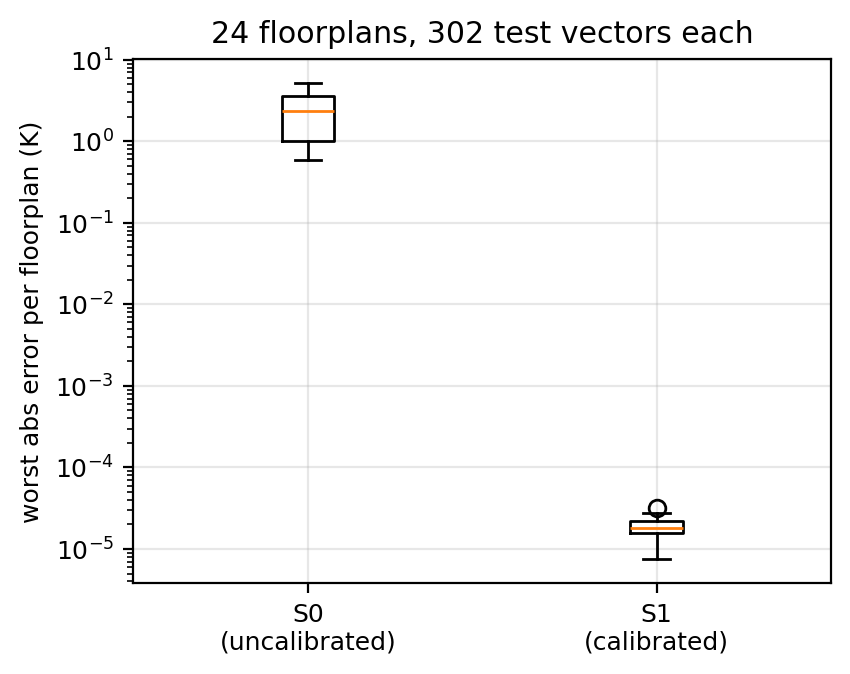
\includegraphics[width=0.5\linewidth]{P2-1_steady_predictor/results/steady_accuracy_stage2.png}
  \caption{Worst error of S0 and S1, as a box over the 24 floorplans (one value per floorplan,
  log scale).}
\end{figure}

\subsection{Compressing $G$ for chips with many cores}
For 8 cores $G$ is at most 1.6\,kB, so compression is not needed. It grows as $N^2$, though,
so we asked whether a smaller form of $G$ would do. The standard way to shrink a matrix is a
\emph{low-rank} approximation: keep only the $r$ largest singular values of $G$ (truncated SVD),
$G \approx U V^\top$ with $U$ of size $n\times r$ and $V$ of size $N\times r$, which stores
$r(n+N)$ numbers instead of $nN$. We compared it with the full S1 on the 8-core floorplans and on a
synthetic 64-core chip (HOM-64, 16$\times$16\,mm).

\begin{center}
\small
\begin{tabular}{@{}l l c c@{}}
\toprule
Chip & Model & Size & Worst error \\
\midrule
8 cores (24 floorplans, median size) & Full S1 & 928\,B & 0.00003\,K \\
 & Low rank, $r=2$ & 360\,B & 12.1\,K \\
 & Low rank, $r=4$ & 720\,B & 12.1\,K \\
 & Low rank, $r=7$ & 1.26\,kB & 3.3\,K \\
\midrule
HOM-64 (64 cores) & Full S1 & 32.8\,kB & 0.00002\,K \\
 & Low rank, $r=2$ & 2.0\,kB & 4.5\,K \\
 & Low rank, $r=8$ & 8.2\,kB & 3.9\,K \\
 & Low rank, $r=32$ & 32.8\,kB & 3.3\,K \\
\bottomrule
\end{tabular}
\end{center}

\textbf{Low rank does not suit heat flow.} Heat spreads locally, so $G$ is a strong diagonal
(each core's self-heating) plus a near-constant package term. A diagonal matrix is full rank, so
cutting the rank throws away self-heating, the largest entries. Even at $r=32$, the same size as
the full matrix, the 64-core chip is 3.3\,K off, and on the 8-core floorplans a useful rank is
already larger than the full $G$. The full S1 stays the right choice: exact, and 32.8\,kB even
at 64 cores.

\subsection{What the prediction looks like}
\begin{figure}[H]
  \centering
  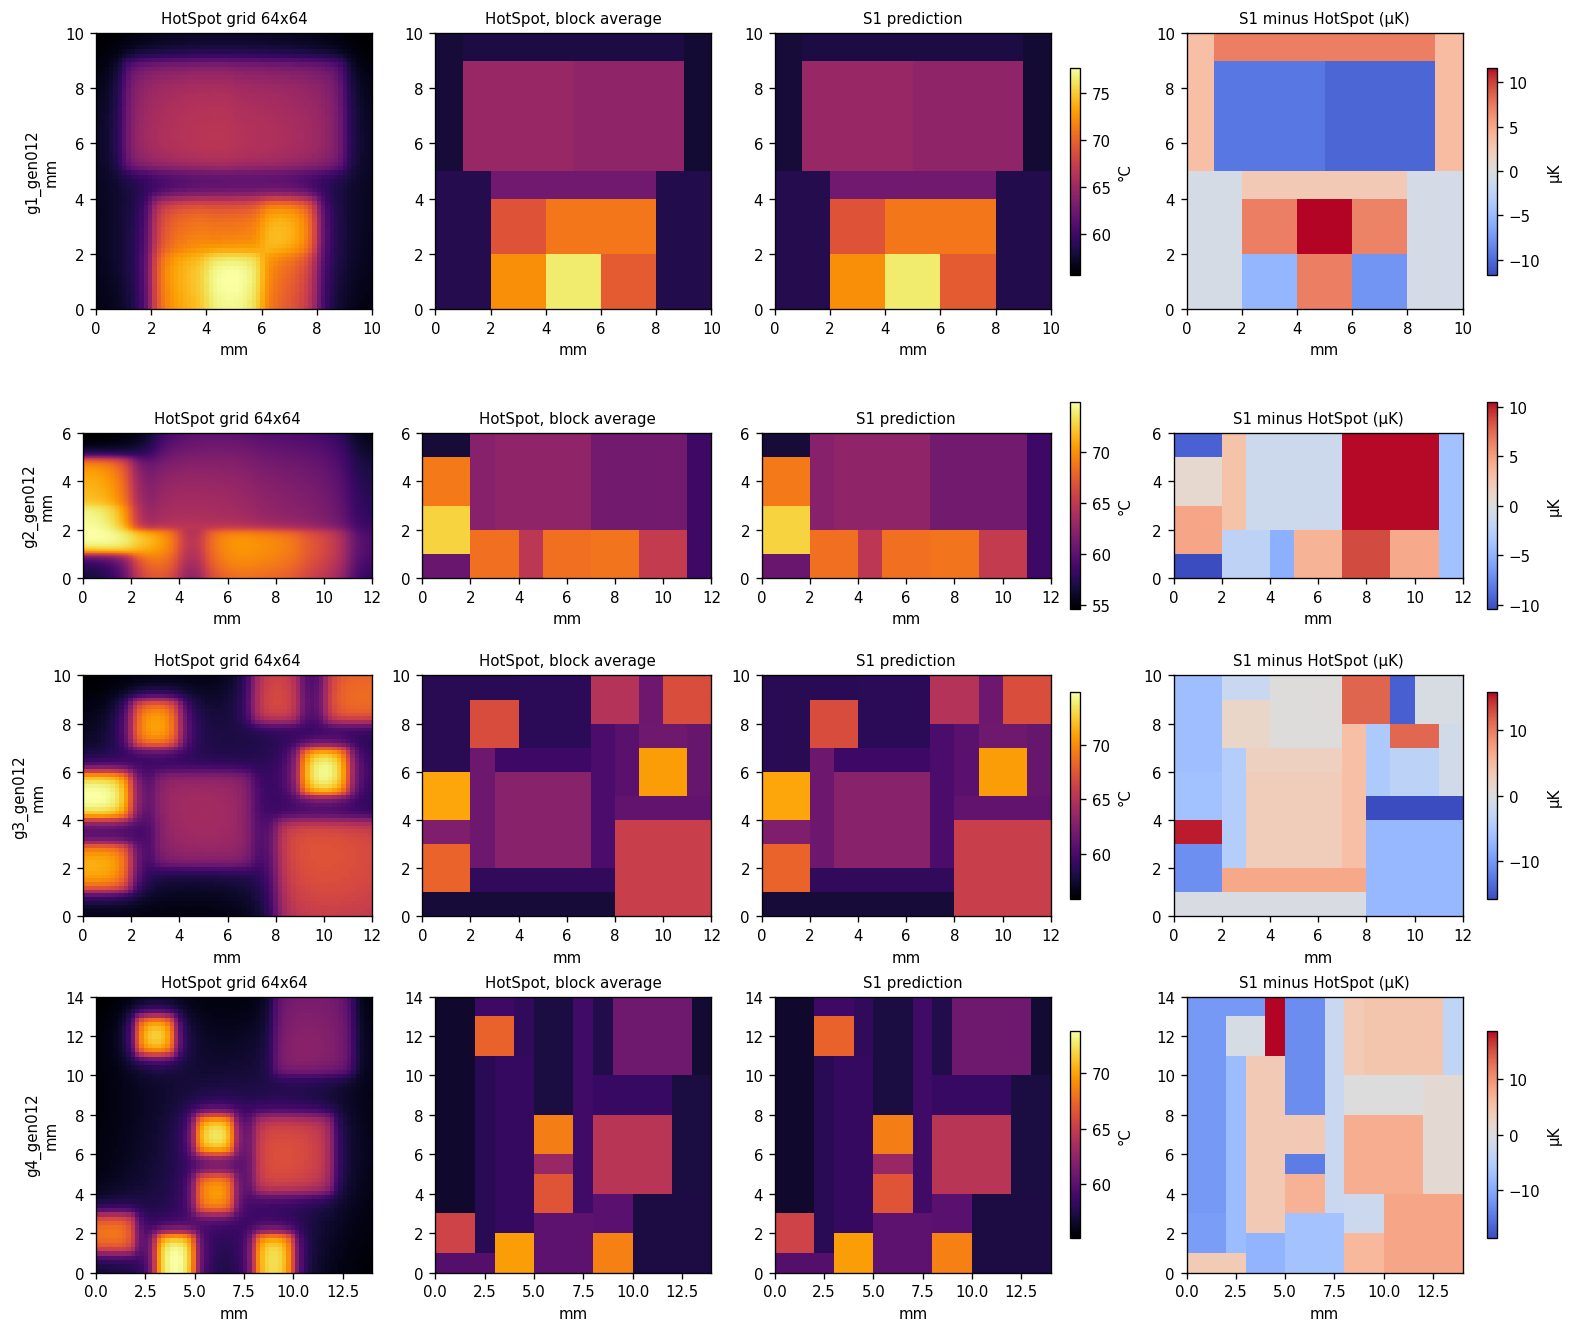
\includegraphics[width=\linewidth]{extended_validation/results/heatmaps.png}
  \caption{One generated floorplan per style, with a random power vector from the test set.
  Columns: HotSpot's $64\times64$ map; HotSpot's block averages; S1's prediction (same colour
  scale); S1 minus HotSpot in \emph{micro}-kelvin. The difference is rounding-sized noise
  (10--19\,$\mu$K at most).}
  \label{fig:s1maps}
\end{figure}

S1's map is indistinguishable from HotSpot's block averages. The first column also shows what any
block-level model misses: the hottest grid cell is 1.3--4.0\,K above the hottest core's average.

%=====================================================================
\section{Why the layout changes $G$}\label{sec:layout}
All 23 given floorplans have the same cores and the same power, yet their $G$ matrices cannot be
swapped. Analysing the calibrated $G$ of all of them against the geometry (no new HotSpot runs)
shows four effects.

\begin{itemize}
  \item \textbf{Edges.} A core on the die edge cannot spread heat outwards: little cores heat
        themselves 8\,\% more on average and up to 27\,\% more. Most given cores (117 of 182) sit on
        an edge.
  \item \textbf{Distance.} Coupling falls steeply over the first 4\,mm (0.63 to 0.15\,K/W) and then
        levels off. Which cores are neighbours decides most of $G$.
  \item \textbf{Die size.} Every core warms the shared spreader and heat sink, a package term of
        0.10--0.14\,K/W, which is smaller on bigger dies.
  \item \textbf{White space keeps the chip cooler.} Peak temperature rises with core coverage
        (correlation $+0.83$). Even with the same die (Style 4), the hottest core ranges from 68.9
        to 72.2\degC\ purely from placement.
\end{itemize}

%=====================================================================
\section{Hot spots inside a core}\label{sec:hotspot}
S1 predicts a core's \emph{average}, but its hottest point is several kelvin higher
(3.3--4\,K, Section~\ref{sec:blockgrid}), and DTM
should protect the real peak. The calibration runs already contain the answer.

\textbf{S1-hot-max.} Each calibration run produces HotSpot's full $64\times64$ temperature map,
so for every grid cell $q$ we have a row of $N$ coefficients $G^\text{cell}_{qj}$: the rise of
cell $q$ per watt in core $j$. Keeping the rows of all cells inside core $c$, the hot spot of $c$
is predicted as
\[ T_\text{hot}(c) = T_\text{amb} + \max_{q\,\in\,c} \sum_j G^\text{cell}_{qj}\,P_j . \]
Because HotSpot is linear, every cell's prediction is exact, so the maximum is exact too, and the
hottest cell is free to move as the power pattern changes. It needs no extra HotSpot runs. The
cost is size: 8 coefficients for every cell inside a core (1{,}134--3{,}823 cells per floorplan,
115\,kB median), so we also tested ways to shrink it:
\begin{itemize}
  \item \textbf{Smaller numbers:} 32-bit storage instead of 64-bit.
  \item \textbf{Coarser grid} ($32\times32$, $16\times16$) and \textbf{low rank} (truncated SVD),
        for comparison.
\end{itemize}
Tested on 23 floorplans with 60 random power vectors each (1{,}380 HotSpot runs); the truth for
each core is its hottest cell.

\begin{center}
\small
\begin{tabular}{@{}l c c c c@{}}
\toprule
Model & Size & Mean error & Worst error & Hottest core right \\
\midrule
Core average (plain S1) & 512\,B & 2.73\,K & 8.96\,K & 50\,\% \\
S1-hot-max, all cells & 115\,kB & 0.000007\,K & 0.00003\,K & 100\,\% \\
\quad 32-bit & 57\,kB & 0.000007\,K & 0.00003\,K & 100\,\% \\
Coarse grid $32\times32$ & 29\,kB & 0.14\,K & 2.8\,K & 95\,\% \\
Coarse grid $16\times16$ & 7.2\,kB & 0.47\,K & 4.7\,K & 85\,\% \\
Low rank, $r=2$ & 29\,kB & 3.4\,K & 11.4\,K & 10\,\% \\
\bottomrule
\end{tabular}
\end{center}

\begin{itemize}
  \item \textbf{The core average underestimates the real peak} by 2.7\,K on average and up to
        9\,K. A limit applied to core averages would let the true hot spot run that much hotter.
  \item \textbf{S1-hot-max is exact} (0.00003\,K worst) with no extra HotSpot runs.
  \item \textbf{32-bit storage halves the model} (57\,kB) with no loss of accuracy.
  \item \textbf{Lossy shortcuts cost far more:} a coarser grid misses the peak (2.8\,K worst at
        $32\times32$), and low rank is worse than the plain core average.
\end{itemize}

%=====================================================================
\section{Scorecard against our targets}
\begin{center}
\small
\begin{tabular}{@{}l c c c@{}}
\toprule
Metric (S1) & Target & Achieved & Status \\
\midrule
Mean error per block & $\le 0.1$\,K & 0.000006\,K & met \\
Error in the peak & $\le 0.2$\,K & 0.00003\,K & met \\
Hottest core right & $\ge 99\,\%$ & 100\,\% & met \\
Time per prediction & $\le 20$\us & 2.6\us & met \\
Model size & $\le 5$\,kB & 512--1{,}600\,B & met \\
\bottomrule
\end{tabular}
\end{center}

%=====================================================================
\section{Implementation status}
\begin{center}
\small
\begin{tabular}{@{}l l@{}}
\toprule
Component & Status \\
\midrule
HotSpot precision patch and dataset (23 given, 3 own, 52 generated floorplans) & done \\
Reference checks (linearity, block vs grid) & done \\
Steady calibration and predictors S0, S1, S1-hot-max, evaluated on 24 floorplans & done \\
Transient predictor and its calibration & next stage \\
\bottomrule
\end{tabular}
\end{center}

%=====================================================================
\section{Changes from the planned scope}
\begin{center}
\small
\begin{tabular}{@{}p{3cm} p{4.4cm} p{7.6cm}@{}}
\toprule
Item & Planned & Done, and why \\
\midrule
HotSpot build & A precision patch & Done as planned: HotSpot prints 6 decimals instead of 2, because our errors are far below its 0.01\,K rounding. \\
Dataset & Our own synthetic floorplans & The 23 given floorplans became the main set, plus 52 generated in the same styles. \\
Hot spots & One hottest cell per core & S1-hot-max over all cells of a core, which is exact and needs no extra runs. \\
\bottomrule
\end{tabular}
\end{center}

%=====================================================================
\section{Future work}
The next stages will extend the predictor to transient temperatures (temperature over time as
power changes), test how robust it is, package it as a tool, and, as the wishlist item, use it for
proactive DTM.

%=====================================================================
\section{LLM assistance disclosure}
LLMs were used to understand HotSpot, for literature review to select appropriate models, to
generate floorplans, to write calibration and testing scripts, and to create this document
using \LaTeX.

%=====================================================================
\begin{thebibliography}{99}\small
\setlength{\itemsep}{2pt}
\bibitem{skadron03} K.~Skadron, M.~R. Stan, W.~Huang, S.~Velusamy, K.~Sankaranarayanan and
  D.~Tarjan, ``Temperature-Aware Microarchitecture,'' in \emph{Proc. ISCA}, 2003.
\bibitem{hotspot} W.~Huang, S.~Ghosh, S.~Velusamy, K.~Sankaranarayanan, K.~Skadron and
  M.~R. Stan, ``HotSpot: A Compact Thermal Modeling Methodology for Early-Stage VLSI Design,''
  \emph{IEEE TVLSI} 14(5):501--513, 2006.
\bibitem{hotspot6} R.~Zhang, M.~R. Stan and K.~Skadron, ``HotSpot 6.0: Validation, Acceleration
  and Extension,'' Univ. of Virginia, Tech. Rep. CS-2015-04, 2015.
\bibitem{huang07} W.~Huang et al., ``An Improved Block-Based Thermal Model in HotSpot 4.0 with
  Granularity Considerations,'' in \emph{Proc. WDDD}, 2007.
\bibitem{blurring} A.~Ziabari, J.-H. Park, E.~K. Ardestani, J.~Renau, S.-M. Kang and
  A.~Shakouri, ``Power Blurring: Fast Static and Transient Thermal Analysis Method for Packaged
  Integrated Circuits and Power Devices,'' \emph{IEEE TVLSI} 22(11):2366--2379, 2014.
\bibitem{coskun09} A.~K. Coskun, T.~S. Rosing and K.~C. Gross, ``Utilizing Predictors for
  Efficient Thermal Management in Multiprocessor SoCs,'' \emph{IEEE TCAD} 28(10), 2009.
\bibitem{zhang18} K.~Zhang, A.~Guliani, S.~Ogrenci-Memik, G.~Memik, K.~Yoshii, R.~Sankaran and
  P.~Beckman, ``Machine Learning-Based Temperature Prediction for Runtime Thermal Management
  Across System Components,'' \emph{IEEE TPDS} 29(2):405--419, 2018.
\bibitem{thermbench} D.~Hang, W.~Yang, K.~Ding, H.~Xin and J.~Wei, ``IC-ThermBench: An Open,
  Progressive Benchmark for Generalizable 2.5D/3D-IC Thermal Learning,'' arXiv:2608.23977, 2026.
\end{thebibliography}

\end{document}
